Debido a la naturaleza de la sucesión de Fibonacci contamos con diferentes formas para expresar un algoritmo para obtener los elementos de la sucesión. A continuación realizaremos una comparación del algoritmo en su presentación usual, es decir, el que calcula el elemento mediante recursividad, y mediante programación dinamica, en sus enfoques Top-Down y Bottom-Up.

\subsection*{Análisis a posteriori}
    Para la realización de nuestra gráfica, se realizó un conteo del número de operaciones realizadas por cada algoritmo para cada entrada n, siendo n el enésimo elemento de la sucesión de Fiboncci. A continuación en las figuras \ref{TablaFiboTop}, \ref{TablaFiboBottom} y \ref{TablaFiboRec}, se presentan los pares ordenados considerados en la gráfica.
    
    \begin{figure}[h!]
        \centering
        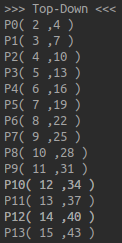
\includegraphics[width=5cm]{Fibonacci/tab-fibo-top.png}
        \caption{Pares ordenados obtenidos para el algoritmo de Fibonacci con programación dinámica utilizando el enfoque Top-Down.}
        \label{TablaFiboTop}
    \end{figure}
    \newpage
    \begin{figure}[h!]
        \centering
        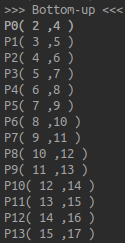
\includegraphics[width=5cm]{Fibonacci/tab-fibo-botttom.png}
        \caption{Pares ordenados obtenidos para el algoritmo de Fibonacci con programación dinámica utilizando el enfoque Bottom-Up.}
        \label{TablaFiboBottom}
    \end{figure}
    
    \begin{figure}[h!]
        \centering
        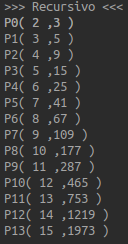
\includegraphics[width=5cm]{Fibonacci/tab-fibo-rec.png}
        \caption{Pares ordenados obtenidos para el algoritmo de Fibonacci en su presentación usual a través de recursividad.}
        \label{TablaFiboRec}
    \end{figure}
    
    \newpage

    Fueron considerados únicamente 14 puntos para cada algoritmo para que siguiera siendo posible apreciar las pequeñas diferencias que presentan los dos enfoques de programación dinámica. Cada uno de los puntos, tiene como abscisa a n, siendo el enésimo elemento de la sucesión de Fibonacci y como ordenadas al número de operaciones realizadas por el algoritmo. Finalmente, observamos en la figura \ref{GraficaFibonacci} la gráfica que representa los pares de puntos obtenidos.
    
    \begin{figure}[h!]
        \centering
        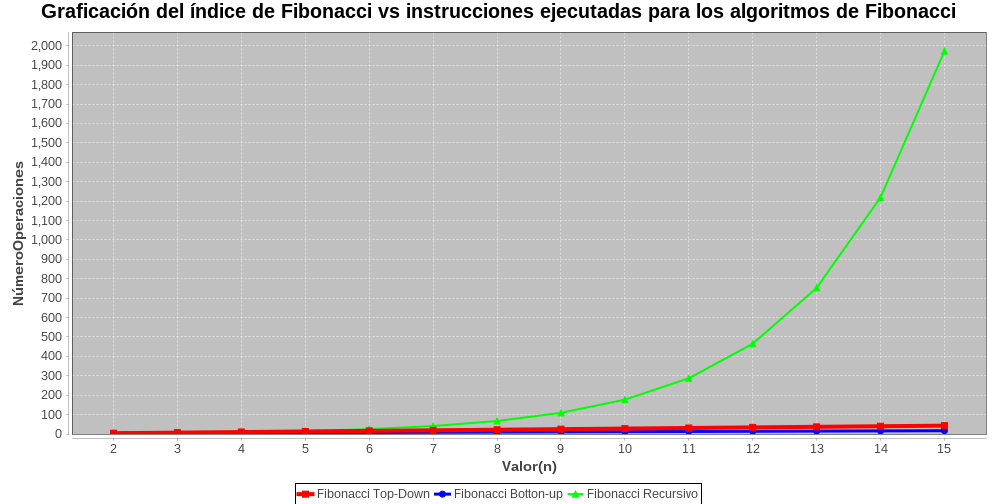
\includegraphics[width=18cm]{Fibonacci/fibo-din-graph.png}
        \caption{Grafica obtenida de la comparación de los algoritmos para el cálculo del enésimo elemento de la sucesión de Fibonacci mediante el conteo del número de operaciones realizadas en cada caso.}
        \label{GraficaFibonacci}
    \end{figure}
    \newpage
    A continuación, en la figuras \ref{GraficaDesmosFiboDinamico} y \ref{GraficaDesmosFiboRecu}, se muestra la comparación de los puntos encontrados experimentalmente para estos algoritmos para el cálculo del enésimo elemento de la sucesión de Fibonacci mediante programación dinámica y con recursividad simple, contra nuestra propuesta de ecuación que describe la complejidad temporal de los mismos.
    
    \begin{figure}[h!]
        \centering
        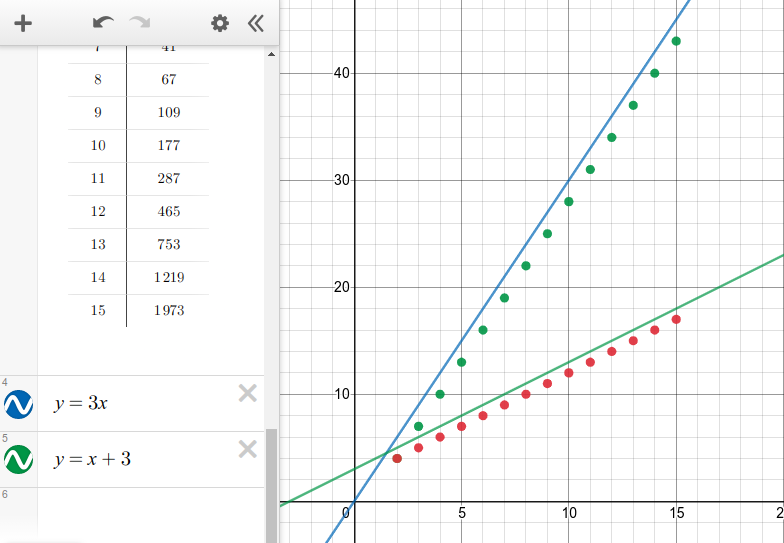
\includegraphics[width=18cm]{Fibonacci/fibo-graph-desm1.png}
        \caption{Representación gráfica de la complejidad temporal de los algoritmos de Fibonacci usando programación dinámica comparada con nuestras propuestas de ecuaciones que los acotan}
        \label{GraficaDesmosFiboDinamico}
    \end{figure}
    
    En la figura \ref{GraficaDesmosFiboDinamico}, los puntos de color verde representan los pares ordenados obtenidos mediante el enfoque Top-Down, mientras que los de color rojo representan los pares ordenados obtenidos con el enfoque Bottom-Up. La recta $y=3x$ es nuestra propuesta de ecuación que acota la complejidad temporal para el enfoque Top-Down, y la recta $y=x+3$ es la propuesta de ecuación que acota la complejidad temporal para el enfoque Bottom-Up. Es particularmente interesante observar que aunque los dos enfoques comparten una complejidad lineal dada por $\Theta(n)$, parece por los resultados experimentales que el enfoque Bottom-Up es más eficiente.
    
    \newpage
    
    \begin{figure}[h!]
        \centering
        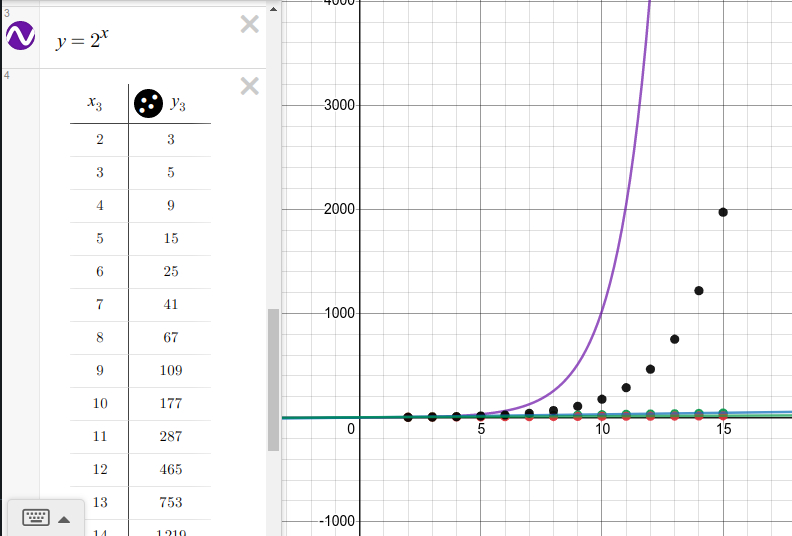
\includegraphics[width=18cm]{Fibonacci/graph-fibo-desm2.png}
        \caption{Representación gráfica de la complejidad temporal del algoritmo de Fibonacci usando su presentación usual de recursividad simple comparada con nuestra propuesta de ecuación que la acota.}
        \label{GraficaDesmosFiboRecu}
    \end{figure}
    
    En la figura \ref{GraficaDesmosFiboRecu}, los puntos en color negro representan los pares ordenados obtenidos por el algoritmo de Fibonacci en su presentación usual. La función $y=2^{x}$ es nuestra propuesta de ecuación que acota la complejidad temporal del algoritmo. Por lo tanto la complejidad temporal esta dada por $\Theta(\phi^{n})$.
    
    Como podemos observar, hay una diferencia abismal entre la cantidad de operaciones realizadas por el algoritmo usando recursividad simple comparado con aquellos que utilizan la programación dinámica para potenciar la eficiencia del cálculo.

\subsection*{Análisis a priori}
    \subsubsection{Fibonacci en su presentación usual}
    Consideremos el pseudocódigo descrito en la figura \ref{PseudocodigoFiboRec} para este algoritmo.
    \begin{figure}[h!]
        \centering
        \begin{verbatim}
            int fiboRec(n:entero)
                if n==0
                    return 0
                else if n==1
                    return 1
                else
                    return fiboRec(n-1)+fiboRec(n-2)
        \end{verbatim}  
        \caption{Pseudocódigo del algoritmo de Fibonacci en su presentación usual.}
        \label{PseudocodigoFiboRec}
    \end{figure}
    \newpage
    A continuación se describe el análisis de complejidad por bloques.
    
    \begin{equation*}
        \left.
            \begin{aligned}
                \left.
                    \begin{aligned}
                        \text{if n==0}\\
                        \text{return 0}\\
                        \text{else if n==1}\\
                        \text{return 1}\\
                    \end{aligned}
                \right\}
                \quad\Theta(1)
                \\
                \left.
                    \begin{aligned}
                        \text{else}\\
                        \text{return fiboRec(n-1)+fiboRec(n-2)}
                    \end{aligned}
                \right\}
                \quad T(n-1)+T(n-2)
                \\
            \end{aligned}
        \right\}
        \quad T(n)=T(n-1)+T(n-2)
    \end{equation*} 
    
    Finalmete, resolviendo la ecuación de recurrencia $T(n)=T(n-1)+T(n-2)$ por el método de ecuación característica, tenemos que la complejidad temporal del algoritmo de Fibonacci en su presentación usual tiene una complejidad temporal $\mathcal{O}(\phi^{n})$.
    
    \subsubsection*{Fibonacci usando programación dinámica con el enfoque Top-Down}
    Consideremos el pseudocódigo descrito en la figura \ref{PseudocodigoFiboTop} para este algoritmo.
    
    \begin{figure}[h!]
        \centering
        \begin{verbatim}
            int fiboTop(n:entero, fibo:tabla)
                if fibo[n] != -1
                    return fibo[n]
                fibo[n] = fiboTop(n-2) + fiboTop(n-1)
                return fibo[n]
        \end{verbatim}  
        \caption{Pseudocódigo del algoritmo de Fibonacci mediante programación dinámica con enfoque Top-Down}
        \label{PseudocodigoFiboTop}
    \end{figure}
    
    A continuación se describe el análisis de complejidad por bloques.
    
    \begin{equation*}
        \left.
            \begin{aligned}
                \left.
                    \begin{aligned}
                        \text{if fibo[n] != -1}\\
                        \text{return fibo[n]}\\
                    \end{aligned}
                \right\}
                \quad\Theta(1)
                \\
                \left.
                    \begin{aligned}
                        \text{fibo[n] = fiboTop(n-2) + fiboTop(n-1)}
                    \end{aligned}
                \right\}
                \quad\Theta(n)
                \\
                \left.
                    \begin{aligned}
                        \text{return fibo[n]}
                    \end{aligned}
                \right\}
                \quad\Theta(1)
                \\
            \end{aligned}
        \right\}
        \quad\Theta(n)
    \end{equation*} 
    
    Finalmente, se concluye que el algoritmo de la sucesión de Fibonacci usando programación dinámica con el enfoque Top-Down tiene una complejidad temporal lineal dada por $\Theta(n)$.
    
    \subsubsection*{Fibonacci usando programación dinámica con el enfoque Bottom-Up}
    Consideremos el pseudocódigo descrito en la figura \ref{PseudocodigoFiboDown} para este algoritmo.
    
    \begin{figure}[h!]
        \centering
        \begin{verbatim}
            int fiboBottom(n:entero, fibo:tabla)
                if n <= 1
                    return 1
                else
                    fibo[0] = 0
                    fibo[1] = 1
                    for i=2 to i<=n do
                        fibo[i]=fibo[i-1]+fibo[i-2]
                return fibo[n]
        \end{verbatim}  
        \caption{Pseudocódigo del algoritmo de Fibonacci mediante programación dinámica con enfoque Bottom-Up}
        \label{PseudocodigoFiboDown}
    \end{figure}
    
    A continuación se describe el análisis de complejidad por bloques.
    
    \begin{equation*}
        \left.
            \begin{aligned}
                \left.
                    \begin{aligned}
                        \text{if n}\leq1\\
                        \text{return 1}
                    \end{aligned}
                \right\}
                \quad\Theta(1)
                \\
                \left.
                    \begin{aligned}
                        \text{else}\\
                        \left.
                            \begin{aligned}
                                \text{fibo[0] = 0}\\
                                \text{fibo[1] = 1}\\
                            \end{aligned}
                        \right\}
                        \quad\Theta(1)
                        \\
                        \left.
                            \begin{aligned}
                                \text{for i=2 to } i<=n \text{ do}\\
                                \text{fibo[i] = fibo[i-1] + fibo[i-2]}\\
                            \end{aligned}
                        \right\}
                        \quad\Theta(n)
                        \\
                        \left.
                            \begin{aligned}
                                \text{return fibo[n]}
                            \end{aligned}
                        \right\}
                        \quad\Theta(1)
                        \\
                    \end{aligned}
                \right\}
                \quad\Theta(n)
                \\
            \end{aligned}
        \right\}
        \quad\Theta(n)
    \end{equation*} 

    Finalmente, se concluye que el algoritmo de la sucesión de Fibonacci usando programación dinámica con el enfoque Bottom-Up tiene una complejidad temporal lineal dada por $\Theta(n)$.